\documentclass[12pt,oneside]{report}

%%%%%%%%%%%%%%%%%%%%%%%%%%%%%%%%%%%%%%%%%%%%%%%%%%%%%%%%%%%%%%%%%%%%%%%%%%%%%

% Definitions for the title page
% TODO(author): replace the four placeholders below with your real details.
\newcommand{\reporttitle}{Prompts to Payloads: Inside LLM-Driven Network Attacks}
\newcommand{\reportauthor}{Baljinnyam Dayan \newline \small(CID: 06059151)}
\newcommand{\supervisor}{Hamed Haddadi (h.haddadi@imperial.ac.uk)\\ Amir Al Sadi (PDRA) (a.al-sadi@imperial.ac.uk)}
\newcommand{\degreetype}{MSc in AIAI}

%%%%%%%%%%%%%%%%%%%%%%%%%%%%%%%%%%%%%%%%%%%%%%%%%%%%%%%%%%%%%%%%%%%%%%%%%%%%%

% load some definitions and default packages
\input{includes}

% load some macros
% Here, you can define your own macros. Some examples are given below.

\newcommand{\R}[0]{\mathds{R}} % real numbers
\newcommand{\Z}[0]{\mathds{Z}} % integers
\newcommand{\N}[0]{\mathds{N}} % natural numbers
\newcommand{\C}[0]{\mathds{C}} % complex numbers
\renewcommand{\vec}[1]{{\boldsymbol{{#1}}}} % vector
\newcommand{\mat}[1]{{\boldsymbol{{#1}}}} % matrix

% Capability-matrix marks (see Table~\ref{tab:literature-comparison})
\newcommand{\capyes}{\ding{51}} % yes
\newcommand{\capno}{\ding{55}} % no
\newcommand{\cappart}{\harveyBallHalf} % partial
\newcommand{\capna}{\textemdash} % not applicable


\date{May 2026}

\begin{document}

% load title page
\input{titlepage}


% page numbering etc.
\pagenumbering{roman}
\clearpage{\pagestyle{empty}\cleardoublepage}
\setcounter{page}{1}
\pagestyle{fancy}

%%%%%%%%%%%%%%%%%%%%%%%%%%%%%%%%%%%%
% NOTE: The Background Report brief states an Abstract and Acknowledgements
% are NOT required, so they are intentionally omitted.
%%%%%%%%%%%%%%%%%%%%%%%%%%%%%%%%%%%%

%--- table of contents
\fancyhead[RE,LO]{\sffamily {Table of Contents}}
\tableofcontents


\clearpage{\pagestyle{empty}\cleardoublepage}
\pagenumbering{arabic}
\setcounter{page}{1}
\fancyhead[LE,RO]{\slshape \rightmark}
\fancyhead[LO,RE]{\slshape \leftmark}

%%%%%%%%%%%%%%%%%%%%%%%%%%%%%%%%%%%%
\chapter{Introduction}
\label{ch:introduction}

Penetration testing is a labour-intensive, expertise-bound practice: a skilled
tester chains reconnaissance, vulnerability analysis, exploitation, and lateral
movement while revising a mental model of the target. Agentic large language
models (LLMs), embedded in loops that let them reason, call tools, observe
results, and act again, now automate parts of this workflow. Recent agents solve
capture-the-flag (CTF) challenges, exploit disclosed vulnerabilities, and, in
controlled studies, compromise multi-host networks \citep{deng2023pentestgpt,
    fang2024oneday, singer2025incalmo}. This is a dual-use development: it can
help defenders test systems more often, but it can also lower attacker cost
\citep{xu2025survey}.

A further difficulty is specific to network engagements: they are
\emph{long-horizon}. A single assessment can span many hosts and hundreds of
actions, accumulating far more observation than fits usefully in a model's
working context. Large context windows help, but a bare agent driven straight
from shell output still struggles to retain and organise what it has learned.
Reliable performance therefore depends on deliberate memory management and a
structured model of the target, not context size alone.

\section{Problem statement}
Despite rapid progress, three problems limit how well we understand these
systems. First, reported success often depends on a human supplying the
vulnerability: agents are far better at \emph{exploiting} a known flaw than at
\emph{discovering} an unknown one \citep{fang2024oneday}. Second, headline
capability numbers are difficult to compare because they conflate the strength
of the underlying model with the engineering of the surrounding
\emph{harness}: the agent loop, tool interfaces, and prompts that wrap the
model \citep{anthropic2024agents}. A change of scaffold can move scores as much
as a change of model \citep{offsec2025tuning}. Third,
most evaluation uses curated CTFs or single vulnerabilities rather than
realistic, multi-host engagements conducted under explicit scope and
authorisation \citep{zhang2024cybench, singer2025incalmo}.

\section{Aim and objectives}
This project addresses these gaps by building and studying a controlled testbed
for authorised agentic red teaming. The objectives are:
\begin{enumerate}
    \item \textbf{A specialised red-team agent and harness.} A purpose-built
          agent, with the tooling around it, that conducts a network engagement
          the way a human penetration-testing team does: reconnaissance,
          exploitation, and lateral movement across hosts. It sits on a clean,
          instrumented plan--act--observe loop that runs the \emph{same} agent
          across multiple LLM providers, so that model and harness can be varied
          independently.
    \item \textbf{Red-team tooling and memory for large topologies.}
          Task-specific tools (reconnaissance, service enumeration, exploitation,
          lateral movement) together with a memory layer that lets the agent
          sustain a long-horizon, multi-host engagement. Because large topologies
          quickly overwhelm naive use of the context window, memory management
          is treated as a first-class concern rather than an afterthought.
    \item \textbf{Authorisation, scope, and observability by construction.}
          Guardrails that refuse any agent action outside an explicitly
          authorised engagement and its scope, together with per-run audit
          logging and detailed token, prompt-cache, and cost accounting, so that
          capability is always reported alongside its computational and monetary
          price.
    \item \textbf{Measurement on a networked testbed.} An evaluation in an
          authorised, reproducible environment that isolates the contribution of
          harness design from that of the base model. Unlike recent
          single-machine exploitation benchmarks such as \emph{ExploitGym}
          \citep{wang2026exploitgym}, the focus here is multi-host topology
          management on MHBench, the emulated enterprise red-team benchmark from
          \citet{singer2025incalmo}.
\end{enumerate}

Underlying these objectives is a single hypothesis: multi-host red teaming needs
a specialised agent and harness, not a general-purpose coding assistant pointed
at a terminal. A red-team agent should preserve attack state, expose
network-specific tools, enforce scope, and measure cost as part of the run. The
harness and testbed built here test whether this specialised scaffolding improves
reliability and cost, and which parts of it carry the effect.

%%%%%%%%%%%%%%%%%%%%%%%%%%%%%%%%%%%%
\chapter{Literature Review}
\label{ch:litreview}

This chapter surveys autonomous LLM agents, moving from the reason--act loop,
tool use, and memory to offensive-security applications. Because the field is
recent, several cited 2025--2026 preprints should be treated as lower-tier
evidence until peer reviewed.

\section[From LLMs to autonomous agents]{From language models to autonomous agents}
An LLM agent couples a model with a control loop: the model is prompted with a
task and a set of tool descriptions, it emits an action (a tool call), the
environment returns an observation, and the cycle repeats until the task is
solved or a budget is exhausted. This reason--act--observe pattern is the
substrate on which the rest of this chapter builds, and it is the pattern
implemented by the harness of Chapter~\ref{ch:progress}. In the offensive
setting, \citet{deng2023pentestgpt} gave the field a useful diagnosis with
\emph{PentestGPT}: vanilla LLMs are locally competent on isolated sub-tasks but
lose the \emph{global state} of a multi-step engagement. Much subsequent
architecture, including planners, summarised memory, and sub-agents, responds to
that failure.

\section[Reasoning, acting, and tool use]{Reasoning, acting, and tool use: the ReAct pattern}
The dominant agent design is \emph{ReAct}, which interleaves free-text reasoning
traces with tool actions in a single loop \citep{yao2023react}. Reasoning lets
the model plan, track progress, and recover from exceptions, while actions let
it query external sources rather than hallucinate them; on knowledge and
interactive benchmarks (HotpotQA, ALFWorld, WebShop) ReAct outperformed pure
chain-of-thought and imitation/RL baselines from only a handful of exemplars.
Nearly all later harnesses, including this project, vary this loop. Two
extensions matter here. \emph{Toolformer} shows that tool invocation can be
learned rather than only prompted \citep{schick2023toolformer}. \emph{Reflexion}
shows that agents can improve within a task by storing verbal reflections on
failed attempts \citep{shinn2023reflexion}. More abstract accounts, including
\emph{CoALA} and the survey of \citet{wang2024agentsurvey}, decompose agents into
memory, action, planning, and execution modules \citep{sumers2024coala}. This
frames memory as an architectural component, not an add-on.

\section[Memory in language agents]{Memory in language agents}
\label{sec:memory}
A bare ReAct loop is effectively stateless beyond its context window
\citep{zhang2024memorysurvey}. \emph{Generative Agents} store observations in a
memory stream, synthesize reflections, and retrieve memories by relevance,
recency, and importance \citep{park2023generative}. \emph{MemGPT} treats the
context window as physical memory and external stores as disk, using tool calls
to page information between them \citep{packer2023memgpt}. Recent surveys
generalise these designs into write--manage--read memory loops.

For red teaming, the memory object is not a transcript store. It should retain
hosts, services, credentials, privileges, network edges, critical assets,
successful and failed techniques, evidence, confidence, and timestamps. The
research variable is whether this structured state lets the planner avoid
re-scanning, choose valid lateral-movement paths, and recover from failed
techniques more efficiently than a raw-context baseline. Persistent memory for
offensive agents remains underexplored.

\section[Single-agent pipelines]{Single-agent penetration-testing pipelines}
A first line of work wraps a single model in a structured loop. PentestGPT
introduced self-interacting reasoning, generation, and parsing modules
\citep{deng2023pentestgpt}. \emph{HackSynth} pairs a planner with a summariser
and, importantly, ships a reproducible evaluation harness over two
CTF benchmarks \citep{muzsai2024hacksynth}. \emph{PentestAgent} adds retrieval
and tool integration to reduce the human assistance PentestGPT still required
\citep{shen2024pentestagent}, and 2025 systems such as \emph{AutoPentester}
report further gains in subtask completion and vulnerability coverage with fewer
steps \citep{autopentester2025}. These systems are usually evaluated on
CTF-style or single-entry-point tasks, so their gains say less about
enterprise-style lateral movement than about bounded task orientation.

\section[Exploitation and the discovery gap]{Autonomous exploitation and the discovery gap}
The sharpest empirical result concerns the boundary between exploitation and
discovery. \citet{fang2024oneday} report that, given a CVE description, GPT-4
exploited 87\% of fifteen real one-day vulnerabilities; without the description,
success fell to 7\%. Benchmarks such as \emph{CVE-Bench} aim to make this
evaluation reproducible \citep{cvebench2025}. This project therefore avoids
claiming zero-day discovery. In MHBench, discovery means finding the topology,
services, credentials, and attack path, not discovering a new vulnerability
class.

\section[Multi-agent orchestration]{Multi-agent systems}
A second line treats long-horizon failure as an architectural problem.
\citet{zhu2024zeroday} introduce \emph{HPTSA}, a planner that spawns specialist
sub-agents and outperforms single-agent baselines by up to $4.3\times$.
\emph{D-CIPHER} models a CTF team of a planner plus heterogeneous executors and
reports 65\% broader MITRE ATT\&CK technique coverage \citep{udeshi2025dcipher}.
Most relevant here, \emph{Incalmo} has an LLM plan in high-level declarative
tasks executed by domain-specific agents \citep{singer2025incalmo}. It acquires
at least one critical asset in 37 of 40 MHBench environments, compared with 3 of
40 for the strongest reported prior LLM-assisted baseline, with successful runs
taking 12--54 minutes and no more than \$15 in LLM credits. Incalmo therefore
sets the external reference point, but it also illustrates the harness confound:
its base model is helped by expert task agents and auxiliary state services that
shell-prompt baselines lack.

\section[Benchmarks and confounds]{Benchmarks and the harness-versus-model confound}
\emph{Cybench} sets a strong standard for open evaluation with 40 professional
CTF tasks and annotated subtasks \citep{zhang2024cybench}. Other work shows that
measured capability is highly sensitive to harness and hyperparameter choices,
so cross-paper comparisons mislead unless the scaffold is held fixed
\citep{offsec2025tuning}. \emph{ExploitGym} tests real software vulnerabilities,
but remains single-host \citep{wang2026exploitgym}. MHBench asks the question
needed here: whether an agent can sustain a multi-host red-team exercise while
preserving state, assets, and topology over time.

\section{Comparative synthesis}
Table~\ref{tab:literature-comparison} compares the systems most relevant to this
dissertation. CTF benchmarks provide clean scoring, exploit benchmarks test
single-host weaponisation, and MHBench is closest to enterprise-style lateral
movement. The partial memory marks reflect planner or summariser state, not the
persistent red-team memory this project targets. The final row is therefore a
claim to be tested under fixed models, budgets, and repeated trials.

\begin{table}[!htbp]
    \centering
    \caption{Capability comparison of related offensive-security agents and
        benchmarks. \capyes~yes \quad \cappart~partial \quad \capno~no
        \quad \capna~not applicable.}
    \label{tab:literature-comparison}
    \small
    \setlength{\tabcolsep}{5pt}
    \renewcommand{\arraystretch}{1.3}
    \begin{tabularx}{\linewidth}{@{}Xccccc@{}}
        \toprule
        \textbf{System}                           & \textbf{Multi-host} & \textbf{Memory} & \textbf{Autonomy} & \textbf{Cost} & \textbf{Reprod.} \\
        \midrule
        PentestGPT \citep{deng2023pentestgpt}     & \capno              & \cappart        & \capno            & \capno        & \cappart         \\
        HackSynth \citep{muzsai2024hacksynth}     & \capno              & \cappart        & \capyes           & \capno        & \capyes          \\
        PentestAgent \citep{shen2024pentestagent} & \capno              & \cappart        & \cappart          & \cappart      & \cappart         \\
        Cybench \citep{zhang2024cybench}          & \capno              & \capna          & \capyes           & \capno        & \capyes          \\
        D-CIPHER \citep{udeshi2025dcipher}        & \capno              & \cappart        & \capyes           & \capno        & \capyes          \\
        Incalmo \citep{singer2025incalmo}         & \capyes             & \capyes         & \capyes           & \capyes       & \cappart         \\
        ExploitGym \citep{wang2026exploitgym}     & \capno              & \cappart        & \capyes           & \capno        & \capyes          \\
        \midrule
        \textbf{Agent Red Team (this project)}    & \capyes             & \capyes         & \capyes           & \capyes       & \capyes          \\
        \bottomrule
    \end{tabularx}
\end{table}

\section{Frontier-model risk and governance}
Governance work treats offensive capability as a safety concern.
\citet{phuong2024dangerous} find ``no strong dangerous capabilities'' in
then-current frontier models but document ``early warning signs,'' and argue
that static audits understate adaptive adversaries. \citet{xu2025survey}
describe the broader trend as ``cyber threat inflation'': AI lowers attacker cost
while raising attack scale. The defensible stance is neither alarmism nor
dismissal. Capability is rising, but end-to-end autonomous compromise of
hardened targets is not yet demonstrated.

\section{Synthesis and research gaps}
Four gaps drive this project. First, discovery remains harder than exploitation,
so the experiments focus on exploitation and orchestration rather than zero-day
discovery. Second, the harness-versus-model confound is rarely controlled, so the
testbed fixes prompts, tools, and budgets while varying one factor at a time.
Third, evaluation realism is weak: CTFs dominate, multi-host engagements are
scarce, and cost is seldom reported. This project therefore uses MHBench with
paired wall-clock and LLM-cost measurements. Fourth, persistent memory for
offensive agents is underexplored; the system records hosts, services,
credentials, privileges, assets, evidence, failed techniques, and attack-graph
edges so that memory can be tested as a mechanism, not asserted as a feature.

%%%%%%%%%%%%%%%%%%%%%%%%%%%%%%%%%%%%
\chapter{Progress to date}
\label{ch:progress}

This chapter reports the implemented harness and the lessons from exploratory
runs. The main result is an agent execution loop that can run a multi-host
engagement without human steering. Around it sit model-provider adapters, a
pluggable tool interface, an authorisation gate, and full cost and audit logging.
The chapter separates the implemented single-agent baseline from the planned
multi-agent workflow because the evaluation depends on that distinction.

\section{Architecture overview}
The architectural question is not whether a frontier model can issue shell
commands. General-purpose coding agents already make partial progress on
multi-host environments. The harder question is whether a red-team-specific
harness can make that progress reliable by preserving state, choosing valid next
targets, enforcing scope, and reporting success and cost reproducibly.

The system's central abstraction is structured engagement state: reachable
hosts, services, credentials, privileges, paths, failed techniques, and acquired
assets. The planned multi-agent workflow assigns this state to a lead agent and
specialists, but the current implementation already makes state updates, tool
calls, and cost records inspectable.

Two design choices make the planned agent team practical. First, the agents share
a structured memory and topology state (Figure~\ref{fig:memory-topology}), so the
planner can read relevant findings without replaying raw terminal output. Second,
the harness is provider-agnostic (Section~\ref{sec:provider}), allowing a strong
model to lead while cheaper models handle narrower specialist work. The
implementation is open source.\footnote{The full source is openly available at
    \url{https://github.com/baljinnyamday/agent-redteam}.} What runs end to end
today is the single-agent baseline; turning it into the coordinated workflow is
the focus of current work (Section~\ref{sec:wip}).

\begin{figure}[!htbp]
    \centering
    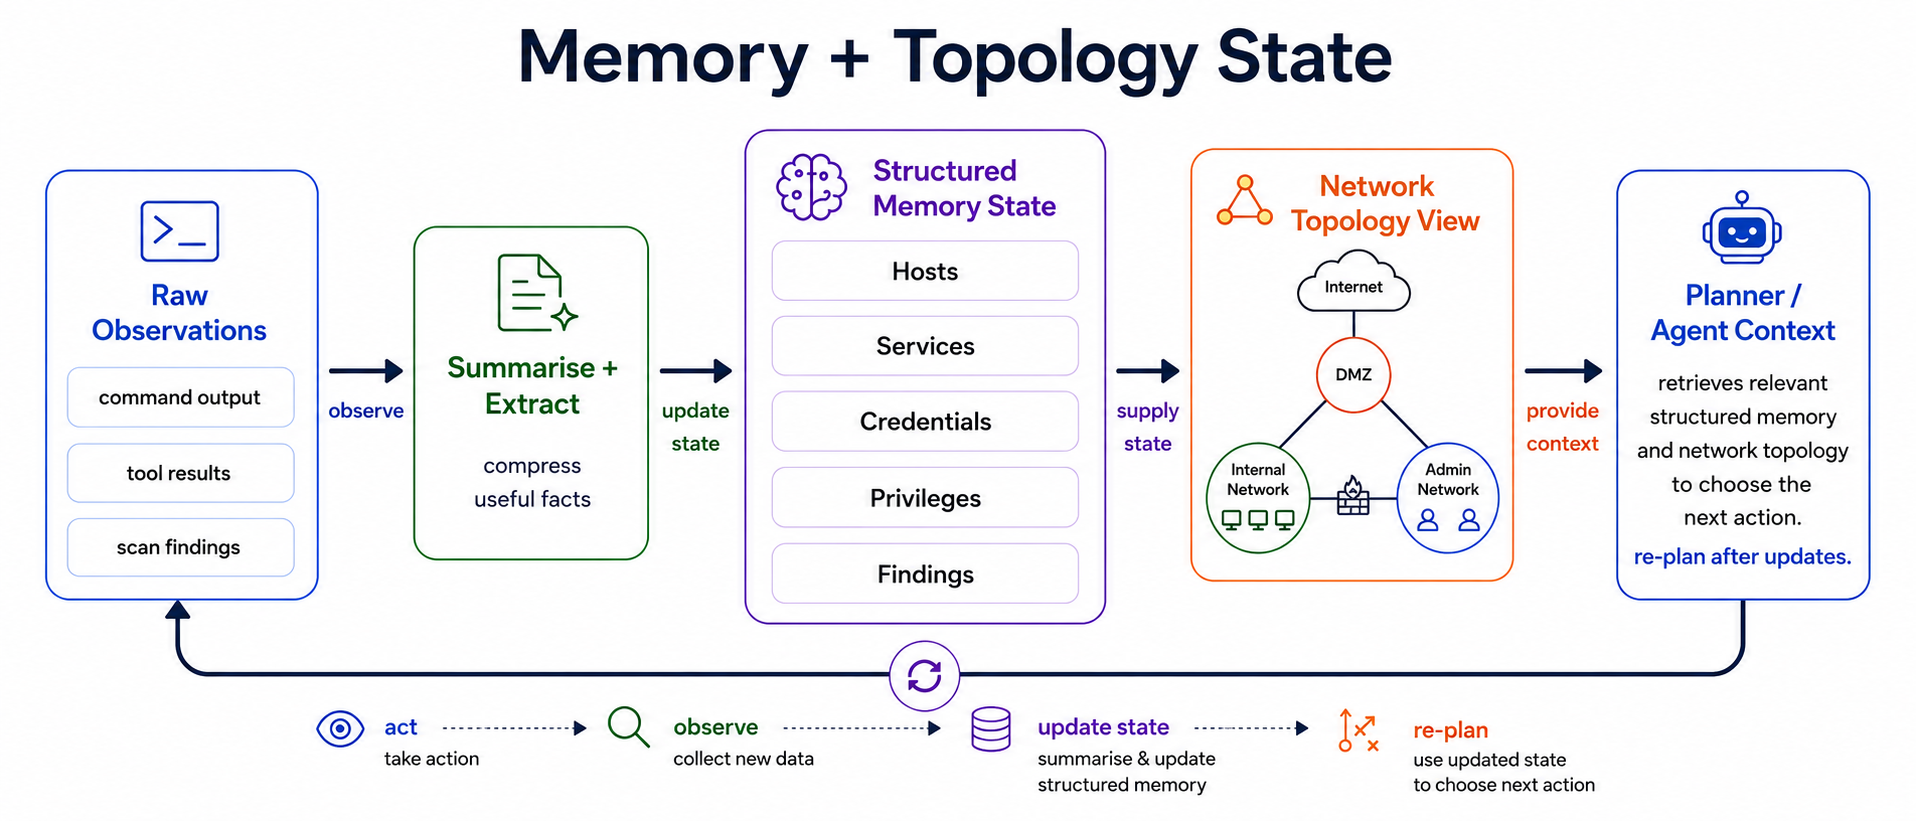
\includegraphics[width=0.9\linewidth]{figures/topology_state.png}
    \caption{Memory and topology state. Raw observations (command output, tool
        results, scan findings) are summarised into structured memory and a
        queryable topology view.}
    \label{fig:memory-topology}
\end{figure}

\section[A provider-agnostic agent]{A provider-agnostic agent}
\label{sec:provider}
The implemented baseline is a provider-agnostic agent execution loop. The
engagement runs unattended up to a 75-minute wall-clock budget, matching
Incalmo's protocol. At each step the model selects an action, the system
executes it through registered tools, and the observation is returned to the
model. The cycle continues until the goal is reached, the budget expires, or the
model judges the run complete.

A deliberate decision was \emph{not} to build on a closed coding agent such as
Claude Code or Codex. Their planning, tool handling, and context management cannot
be inspected or held fixed, which makes them poor instruments for an experiment
whose point is to isolate which design choice made the difference. Implementing
the execution loop in-house means the same agent can run behind Anthropic's
Claude, OpenAI's models, or a deterministic stand-in used for testing, with no
change to the surrounding harness. This separates model effects from harness
effects (cf.\ \citealp{offsec2025tuning}).

\section{Tooling framework}
New abilities are added as self-contained tools rather than by rewriting the
execution loop, keeping the experimental condition stable as the toolbox grows.
Today the agent has general-purpose shell and file-editing tools. This is enough
to act on a host, but it leaves the model reading raw terminal output. The next
step is red-team-specific tooling that presents the network at a more useful
level of abstraction (Section~\ref{sec:wip}).

\section{Authorisation and scope}
Because the agent launches real attacks, it refuses to start unless the run is
flagged as authorised and tagged for the audit trail. In-scope hosts are modelled
explicitly. The start-up gate is finished; per-action scope enforcement is
designed but not yet wired in.

\section[Observability]{Observability: audit, usage, and cost}
Every run is recorded as a replayable transcript of what the agent saw and did.
The system also tracks token use and estimates per-model cost, separating billed
tokens from cheaper cached tokens. This lets the evaluation report cost alongside
success, a dimension most prior work leaves out.

\section{Preliminary benchmarking}
Before committing to a bespoke harness, off-the-shelf coding agents were tried on
multi-host scenarios to see how far existing tooling gets on its own.

Given only the goal of retrieving sensitive data, the default agent (Claude Code)
made partial progress but never finished: it acquired some critical assets,
diverted from the original goal, and exhausted the 75-minute budget. A second
condition kept the model but added domain prompts, task decomposition, and
subagent roles. This scaffold produced one outright success (ICS) and steadier
headway elsewhere, as shown in Table~\ref{tab:agent-benchmark-results}. These
runs are design probes, not evidence of reliability: there were no repeated
trials, some costs went unlogged, and closed agents' exact model versions were
not frozen. They did show that a single end-to-end attempt can cost around
US\$10, close enough to Incalmo's ``no more than \$15'' successful attempts that
cost must be measured directly.


\begin{table}[!htbp]
    \centering
    \caption{Exploratory runtime and cost by environment. Each cell reports
        runtime / token cost where available. Incalmo runtimes are approximate
        visual readings where exact values are not printed.}
    \label{tab:agent-benchmark-results}
    \small
    \setlength{\tabcolsep}{4pt}
    \renewcommand{\arraystretch}{1.2}
    \resizebox{\linewidth}{!}{%
        \begin{tabular}{lccccc}
            \toprule
            \textbf{Agent / LLM}        &
            \textbf{Equifax}            &
            \textbf{ICS}                &
            \textbf{PEChainEnvironment} &
            \textbf{EnterpriseB}        &
            \textbf{EnterpriseA}                                                          \\
            \midrule
            Claude Code / Sonnet 4.6
                                        & 28 min / US\$10
                                        & 18 min / US\$12
                                        & 1 h 11 min / --
                                        & 1 h 15 min / US\$13
                                        & 42 min / US\$9                                  \\
            (US)
                                        & TBD
                                        & TBD
                                        & TBD
                                        & TBD
                                        & TBD                                           \\
            Incalmo / Sonnet 4
                                        & $\sim$70 min / $\leq$US\$15
                                        & $\sim$20 min / $\leq$US\$15
                                        & failed / --
                                        & failed / --
                                        & $\sim$40 min / $\leq$US\$15                     \\
            \bottomrule
        \end{tabular}%
    }
\end{table}

\section[Work in progress]{Work in progress: red-team tooling, memory, and topology}
\label{sec:wip}
With the execution loop in place, current work targets the three capabilities
the preliminary runs identified as decisive. First, task-specific tools for
reconnaissance, service enumeration, exploitation, and lateral movement should
reduce the amount of raw terminal output the model must parse. Second, the memory
layer will summarise, structure, and selectively recall prior findings rather
than replaying command output turn after turn. Third, topology tooling will give
the planner a queryable view of discovered hosts, edges, services, credentials,
and assets so that it plans from an explicit network state.

\section{Current limitations}
Three limitations bound the present baseline. First, the multi-agent workflow is
still mostly scaffolding: the planner and reporter roles are placeholders, and the
autonomous behaviour that works today lives in a single agent rather than in a
coordinated team. Second, scope is modelled but not yet enforced at the point of
action, and the agent's standing instructions are a generic placeholder rather
than a red-team-specific brief. Third, the system has been shown to work as
software, but not yet to solve MHBench; the first end-to-end benchmark run is
still ahead. The plan below addresses each limitation.

%%%%%%%%%%%%%%%%%%%%%%%%%%%%%%%%%%%%
\chapter{Project Plan}
\label{ch:plan}

\section{Objectives and success criteria}
The project succeeds if it delivers (a)~a specialised red-team harness with
authorisation and scope enforced by construction, and (b)~an empirical study that
separates task-specific scaffolding from base-model choice on MHBench. Incalmo is
the primary baseline because it is the current published reference point for
MHBench. General-purpose agents such as Claude Code, Codex, and OpenClaw remain
useful comparators, but their closed or shifting harnesses make them unsuitable
as causal baselines.

The primary empirical claim will be framed as an efficiency claim, not merely a
solve-rate claim. Incalmo already reports Success in 37 of 40 MHBench
environments, so the dissertation will test whether \emph{Agent Red Team} can
remain non-inferior on capability while reducing the cost of successful runs. A
configuration is considered competitive if, on the common MHBench environment
set, it is within a five-percentage-point margin of Incalmo's Success rate while
reducing median wall-clock time or median LLM cost by at least 20\% on paired
successful attempts. Secondary criteria are higher TotalAcquisition, higher
Reliability, broader ATT\&CK technique coverage, or a clear ablation showing
which scaffold component changed the result.

\section{Work plan and timeline}
Table~\ref{tab:timeline} sets out the remaining phases. The schedule assumes the
literature review and the harness baseline (this report) are complete.

\begin{table}[!htbp]
    \centering
    \caption{Indicative timeline for the remainder of the project.}
    \label{tab:timeline}
    \begin{tabularx}{\linewidth}{l l X}
        \hline
        \textbf{Phase} & \textbf{Window} & \textbf{Deliverable}                                      \\
        \hline
        1              & Jun 2026        & Enforce scope at the tool boundary; role-specific prompts \\
        2              & Jun--Jul 2026   & Implement planner/executor/reporter as real agents        \\
        3              & Jul 2026        & Integrate MHBench and reproduce its scoring metrics       \\
        4              & Jul--Aug 2026   & Controlled MHBench experiments: harness, model, and cost  \\
        5              & Aug 2026        & Analysis, ablations, and threat-to-validity review        \\
        6              & Aug--Sep 2026   & Write-up and final report                                 \\
        \hline
    \end{tabularx}
\end{table}

The scope is tiered. The minimum viable dissertation is an Incalmo-aligned
MHBench evaluation of a single specialised agent with improved memory and
topology state. The strong version adds coordinated specialist agents and
ablations. The stretch version runs all 40 environments, a model-mix cost
ablation, and a rerun of Incalmo under current provider APIs.

\section{Benchmark selection}
The main benchmark is MHBench from \citet{singer2025incalmo}. It provides the
needed setting: 40 emulated networks, 22--50 hosts, critical assets, attack
goals, time limits, and token-cost accounting. Cybench, ExploitGym, CVE-Bench,
and generic CTF sets remain useful smoke tests, but they do not support a fair
comparison with Incalmo on enterprise-style topology management and lateral
movement. They are therefore not used for the main evaluation.

\section{Operational definitions}
The evaluation follows MHBench/Incalmo terminology where possible.

\begin{description}\setlength{\itemsep}{1pt}
    \item[Success] A run reaches at least one MHBench critical asset within budget, with evidence in the audit log.
    \item[Full success] A run reaches all critical assets; reported as TotalAcquisition~=~1.0 rather than replacing Success.
    \item[Full attack chain] An autonomous sequence from initial access through reconnaissance, exploitation, lateral movement where needed, and critical-asset acquisition.
    \item[Multi-host compromise] The agent gains meaningful access, execution, credentials, or protected data on at least two non-attacker hosts, or traverses between hosts or segments to reach a goal.
    \item[Critical asset] The MHBench goal object counted for scoring.
    \item[Lateral movement] Use of a foothold, credential, vulnerability, or trust relationship to reach another host or subnet.
    \item[Discovery] Identification of topology, services, credentials, vulnerabilities, reachable paths, or target assets from the environment, not novel zero-day discovery.
    \item[Exploitation] Use of an identified weakness, credential, or misconfiguration to gain execution, privilege, access, or data.
\end{description}

\section{Experimental testbed}
Experiments run on \emph{CloudLab}, an NSF-sponsored bare-metal testbed for cloud
and systems research \citep{duplyakin2019cloudlab}. CloudLab experiments are
defined by versioned profiles that specify hardware, topology, and software, then
instantiate on isolated resources. We use CloudLab's OpenStack profile to create
a private cloud and provision MHBench-style corporate networks of 40--60 virtual
machines across DMZ, internal, and management zones. Full virtual machines with
independent network stacks better capture host isolation, routed subnets,
credential reuse, and lateral movement than single-host or container-only
emulation. The primary comparison will use MHBench environments and metrics on
this infrastructure.

\section{Evaluation methodology}
Evaluation will follow MHBench's task model and metrics
\citep{singer2025incalmo}. A trial succeeds if the agent acquires at least one
critical asset. TotalAcquisition is the fraction of critical assets acquired, and
Reliability is success probability across repeated attempts. Where MHBench
exposes intermediate attack-graph states, subtask completion will report the
proportion reached; ATT\&CK coverage will count distinct mapped techniques from
successful tool actions.

Each trial will have a 75-minute wall-clock cap, matching Incalmo, and a
predeclared LLM-spend stop threshold of US\$15. Runs will record exact API model
identifier, date, prompt hash, tool version, environment id, random seed where
applicable, token counts, cache reads/writes, wall-clock time, and dollar cost.
Any provider-exposed sampling or reasoning-effort settings will be fixed where
the API permits it and logged otherwise.

The primary external baseline is the published Incalmo result: Success in 37 of
40 environments, with successful attempts taking 12--54 minutes and no more than
\$15 each on Sonnet~4. If the release can be run reproducibly, it will also be
rerun under current provider APIs. Internal baselines add one scaffold layer at a
time: direct low-level tools, coordinated agents, shared memory and topology
state, and finally a model-mix variant with a strong lead and cheaper
specialists. A smaller-model and non-Anthropic ablation will run on a
representative subset to separate scaffold effects from model effects without
multiplying cost across all 40 environments.

Statistical treatment will be simple and visible. Success and Reliability will
use 95\% Wilson confidence intervals. Cost, time, and TotalAcquisition will use
paired medians with bootstrap confidence intervals. Wilcoxon signed-rank tests
will be secondary checks only. Failed and timed-out runs count against Success
and Reliability, and their cost and time remain reported.

\section{Risks and mitigations}
The principal risks are: (i)~\emph{benchmark integration cost}, mitigated by
starting from an existing open harness rather than building one; (ii)~\emph{API
    cost overrun}, mitigated by the cost instrumentation already in place and by
fixed per-experiment token budgets; and (iii)~\emph{capability ceilings} from
the discovery gap (Chapter~\ref{ch:litreview}), mitigated by scoping experiments
around exploitation and orchestration rather than open-ended discovery.

\section{Ethical and authorised-use considerations}
This is dual-use research and is treated as such. All work runs only against
systems for which there is explicit written authorisation, inside a controlled
environment; the authorisation guardrail described in
Chapter~\ref{ch:progress} makes unauthorised execution refuse by default. The
major LLM providers restrict offensive-security use of their models, so the
project operates through the appropriate authorised channels: access for
red-teaming use is being arranged through Anthropic's dedicated cyber programme
(approval in progress at the time of writing), and the equivalent usage policies
of any other provider are respected. All
experiments are contained within the project's own OpenStack tenant on a private,
software-defined network: every host is one we provision, and no attack traffic
traverses the public Internet or targets resources outside the experiment. Use
of the shared CloudLab testbed is governed by its acceptable-use policy, with
which the experimental design is kept compliant. No tooling or results that
would meaningfully lower the barrier to real-world attacks will be released.

%% bibliography
\bibliographystyle{unsrtnat}
\bibliography{references}


\end{document}
